\section{Conclusion}

Among the test results obtained, there were no relevant differences between the results 
of the models, with an exception of KNN, which had the worst result, but still, not bad. 
A probable cause of this performance of KNN, it is that there are probably a data skewness, 
since the "nature" of KNN, will preferentially classify the data located at the side 
containing more elements, the evidence to it is in the table (4), since there is a 
good classification performance in one of the classes, what suggests that this class 
is more numerous, distorcing the remaining class classification.

This similarity on the results between linear and non-linear methods, means that 
the classes "success" and "failure" are linearly or approximately linearly separable. 
Therefore, it favors the choice of simplest models of less computational cost. 
According to the generated test, the best model was the Quadratic SVM. On the other hand,
that performance was only superior in one hit in comparison with the LDA model. The latter
can be trained with a lot less time and generate equivalent results. 

Like KNN, other models had more considerable errors in one of the classes. The Logistic
Regression had a correct rate smaller in the class "success" than in the "failure" class.
Meanwhile, in the decision trees algorithms, the situation is inverted. The algorithms 
presenting a better trade-off in the class classification were the LDA and the 
Quadratic SVM, with a difference around two percentual points between the correct 
classification rates. It is important to state that the tree is quite efficient with $N>2$ 
classes, since its behavior is intuitive. It simply check conditions in sequence
based on the predictors, which are the decision rules, and link the response of those 
conditions to a certain class at the final step. One good advantage of this method is that it 
doesn't require much data pre-processing.

Having raised these considerations, we conclude that the model with the best
trade-off is the LDA, as its results with respect to corrected classified rates and 
time of training are better than the results of other traditional methods. Its 
corrected classified rate was not discrepant between classes, besides being equiparable 
to the non-linear method with the best performance on the test set. The only caution would 
be if it was necessary to often remodel the methods as more data were to be added.
To this specific situation, the Decision Tree with 10 nodes would be recommended, in order to be 
more agile in the training phase with a large data set.

\section*{Appendix}

\begin{figure}[htbp!]
  \centerline{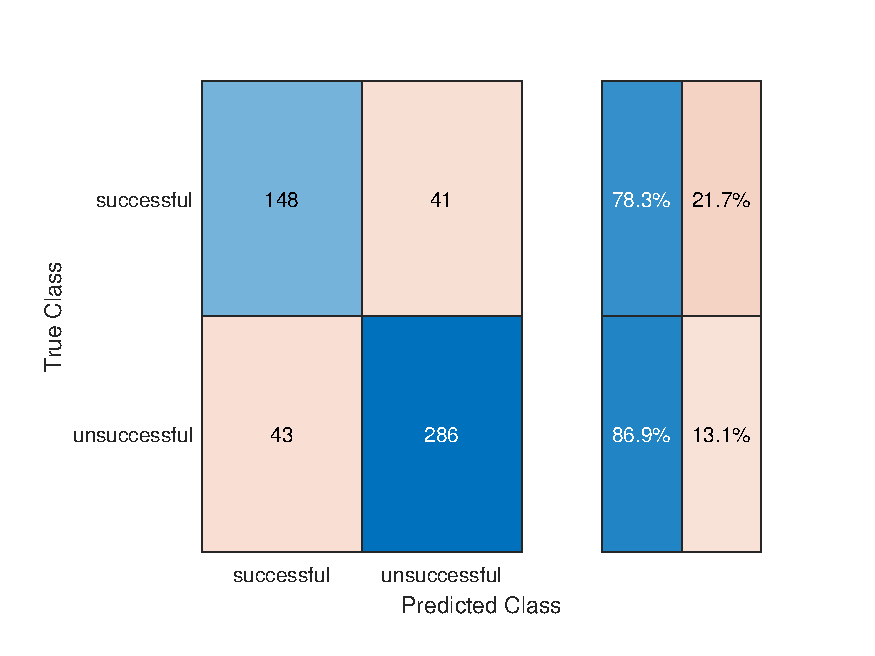
\includegraphics[width=0.3\textwidth]{../../code/hw3/matlab/figures/LR_confusion.pdf}}
  \caption{LR confusion matrix.}
  \label{fig:LR_confusion}
\end{figure}

\begin{figure}[htbp!]
  \centerline{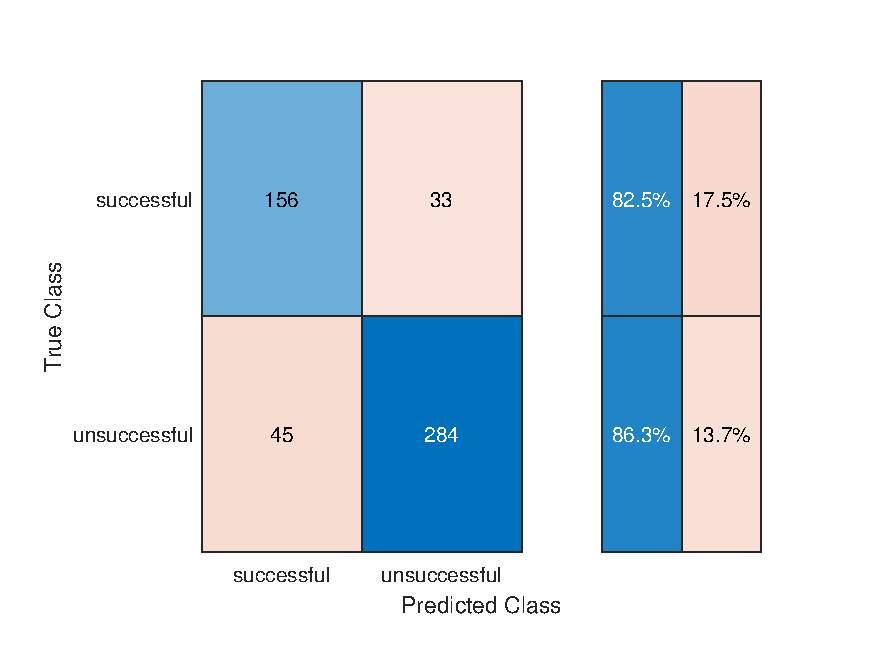
\includegraphics[width=0.3\textwidth]{../../code/hw3/matlab/figures/LDA_confusion.pdf}}
  \caption{LDA confusion matrix.}
  \label{fig:LDA_confusion}
\end{figure}

\begin{figure}[htbp!]
  \centerline{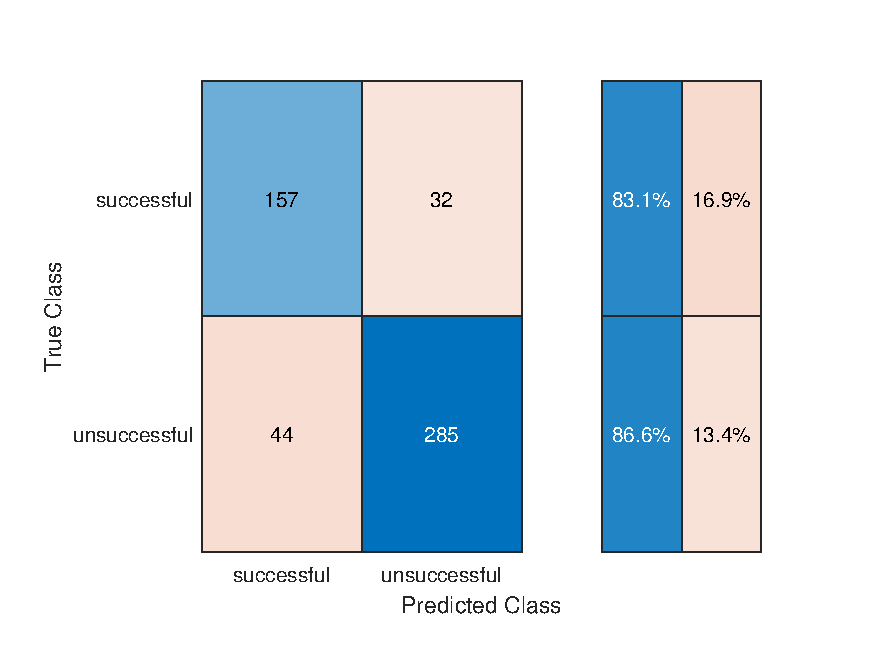
\includegraphics[width=0.3\textwidth]{../../code/hw3/matlab/figures/SVM_confusion.pdf}}
  \caption{SVM confusion matrix.}
  \label{fig:SVM_confusion}
\end{figure}

\begin{figure}[htbp!]
  \centerline{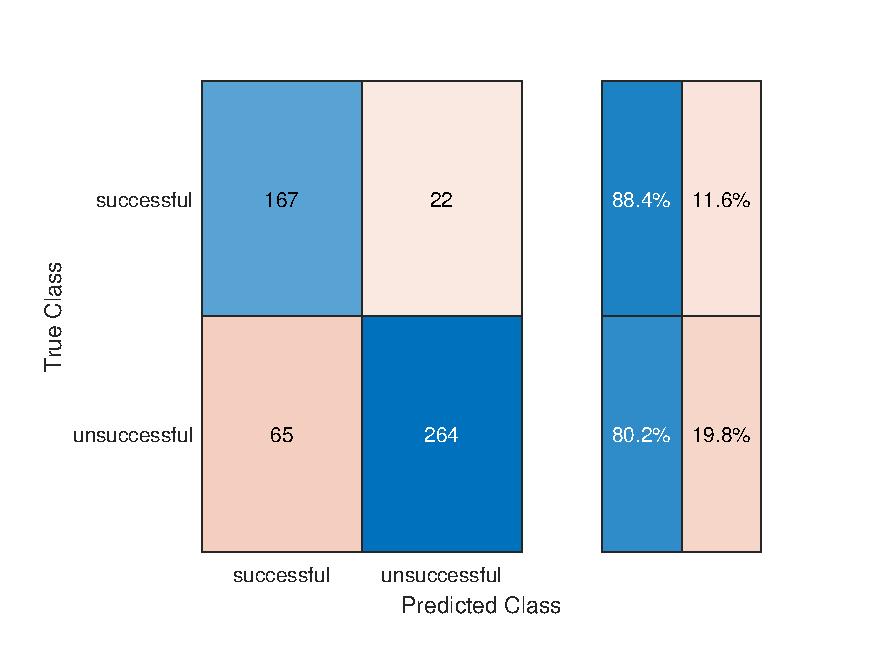
\includegraphics[width=0.3\textwidth]{../../code/hw3/matlab/figures/TREE_10_confusion.pdf}}
  \caption{TREE 10 confusion matrix.}
  \label{fig:TREE_10_confusion}
\end{figure}

\clearpage 

\begin{figure}[htbp!]
  \centerline{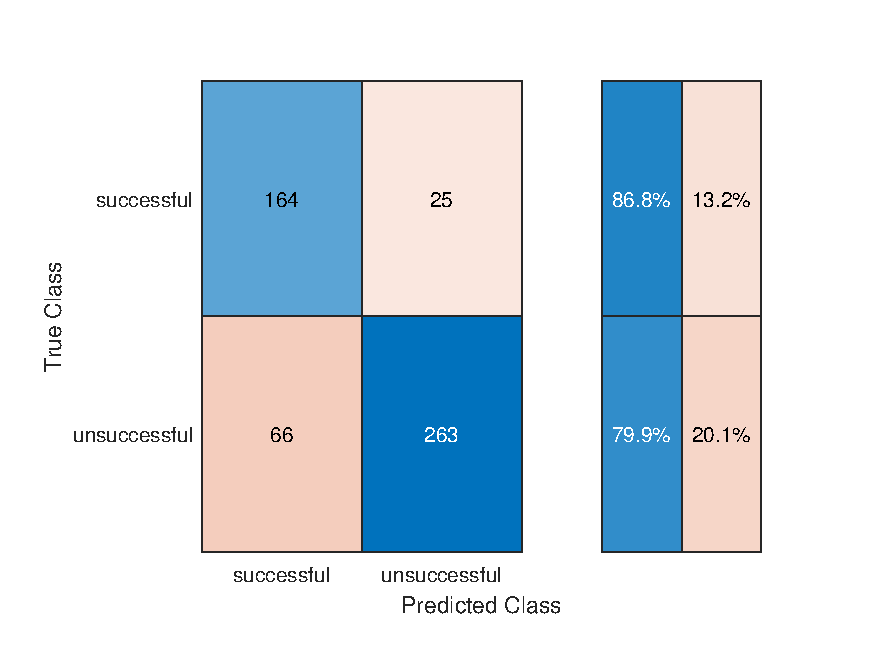
\includegraphics[width=0.3\textwidth]{../../code/hw3/matlab/figures/TREE_100_confusion.pdf}}
  \caption{TREE 100 confusion matrix.}
  \label{fig:TREE_100_confusion}
\end{figure}

\begin{figure}[htbp!]
  \centerline{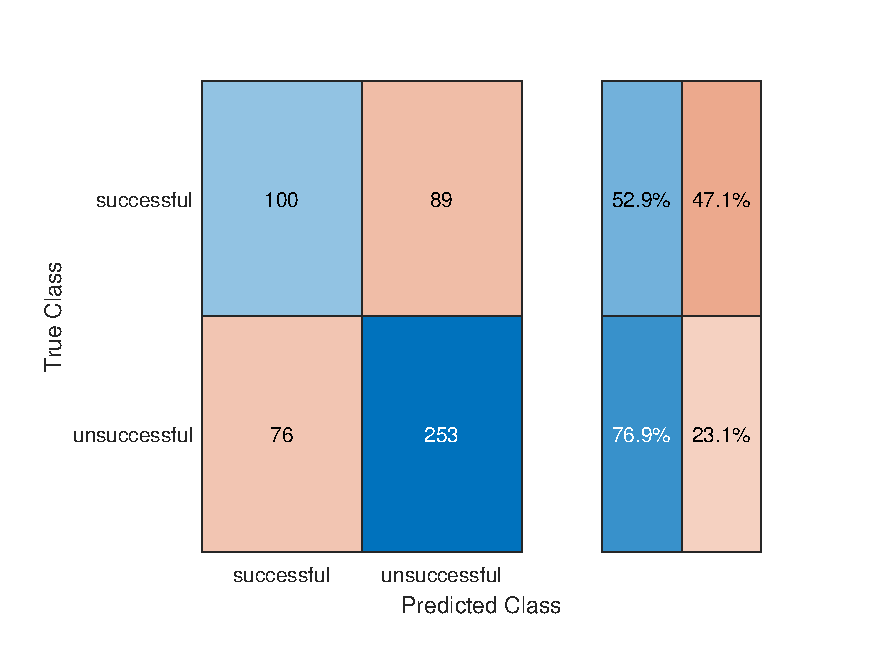
\includegraphics[width=0.3\textwidth]{../../code/hw3/matlab/figures/KNN_1_confusion.pdf}}
  \caption{KNN 1 confusion matrix.}
  \label{fig:KNN_1_confusion}
\end{figure}


\begin{figure}[htbp!]
  \centerline{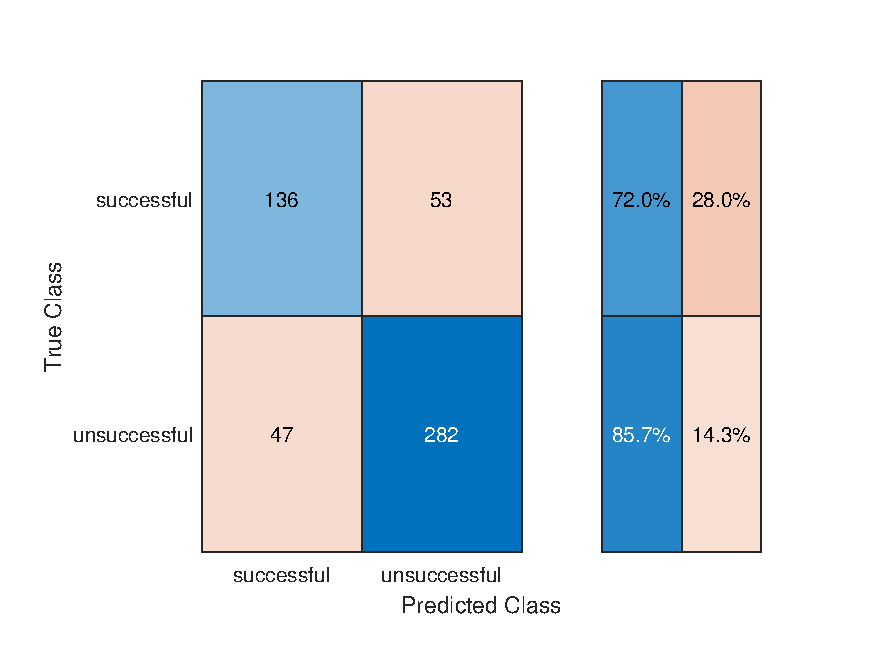
\includegraphics[width=0.3\textwidth]{../../code/hw3/matlab/figures/KNN_50_confusion.pdf}}
  \caption{KNN 50 confusion matrix.}
  \label{fig:KNN_50_confusion}
\end{figure}
